\section{Diseño del Sistema y Arquitectura}
\label{sec:system-design}

\subsection{Arquitectura Centrada en la Configuración}
\label{sec:config-centric-architecture}

La experimentación en este proyecto es \emph{primero el esquema}. En lugar de exponer banderas con validación laxa, la topología del modelo, la familia del optimizador, los límites de entrenamiento y la telemetría pasan por un único documento de configuración validado, lo que reduce la ambigüedad al reproducir resultados y permite que muchas arquitecturas compartan una misma interfaz operativa.

El contrato autoritativo es \path{src/schema.yaml}, un esquema JSON modular cuyos módulos bajo \path{src/schema/} cubren los bloques de modelo, clase de modelo, tokenizer, optimizador, SBERT, entrenamiento y datasets. Los objetos de primer nivel son \texttt{base\_model}, \texttt{tokenizer}, \texttt{model\_class}, \texttt{model}, \texttt{training}, \texttt{image}, \texttt{vision\_dataset} y \texttt{text\_dataset}.

\paragraph{Clase de modelo.} El campo \texttt{model\_class} selecciona entre tres variantes:
\begin{itemize}[leftmargin=*]
    \item \textbf{\texttt{frankenstein\_text\_encoder}}: encoder de arquitectura mixta con toda la gama de mezcladores de secuencia, MoE y normalización avanzada, entrenado con masked language modeling.
    \item \textbf{\texttt{frankenstein\_text\_decoder}}: decoder causal autorregresivo para generación de siguiente token; el runtime fuerza el enmascaramiento de decoder.
    \item \textbf{\texttt{frankenstein\_vit}}: Vision Transformer sobre parches de imagen para predicción de parches enmascarados, clasificación y segmentación; el runtime fuerza el enmascaramiento de encoder y la configuración requiere los bloques \texttt{image} y \texttt{vision\_dataset}.
\end{itemize}

\paragraph{Modo de entrenamiento.} \texttt{model.dims.mode} controla el enmascaramiento: \texttt{encoder} usa atención bidireccional para masked language modeling y \texttt{decoder} usa enmascaramiento causal para predicción autorregresiva.

\paragraph{Selección de mezcladores.} \texttt{model.dims.layer\_pattern} es una lista ordenada de identificadores de mezclador tomados de las ocho familias descritas en la Sección~\ref{sec:architecture-taxonomy}; el esquema fija los identificadores aceptados y la enumeración completa aparece en la Figura~\ref{fig:comprehensive-taxonomy} y el Apéndice~\ref{sec:annex-summary-tables}.

\paragraph{Selección de optimizador.} \texttt{training.optimizer.optimizer\_class} selecciona una de veinticuatro familias de optimizadores, resumidas en la Sección~\ref{sec:optimizer-families} y detalladas en el Apéndice~\ref{sec:annex-optimizers}.

\begin{figure}[t]
\centering
\fitfigure{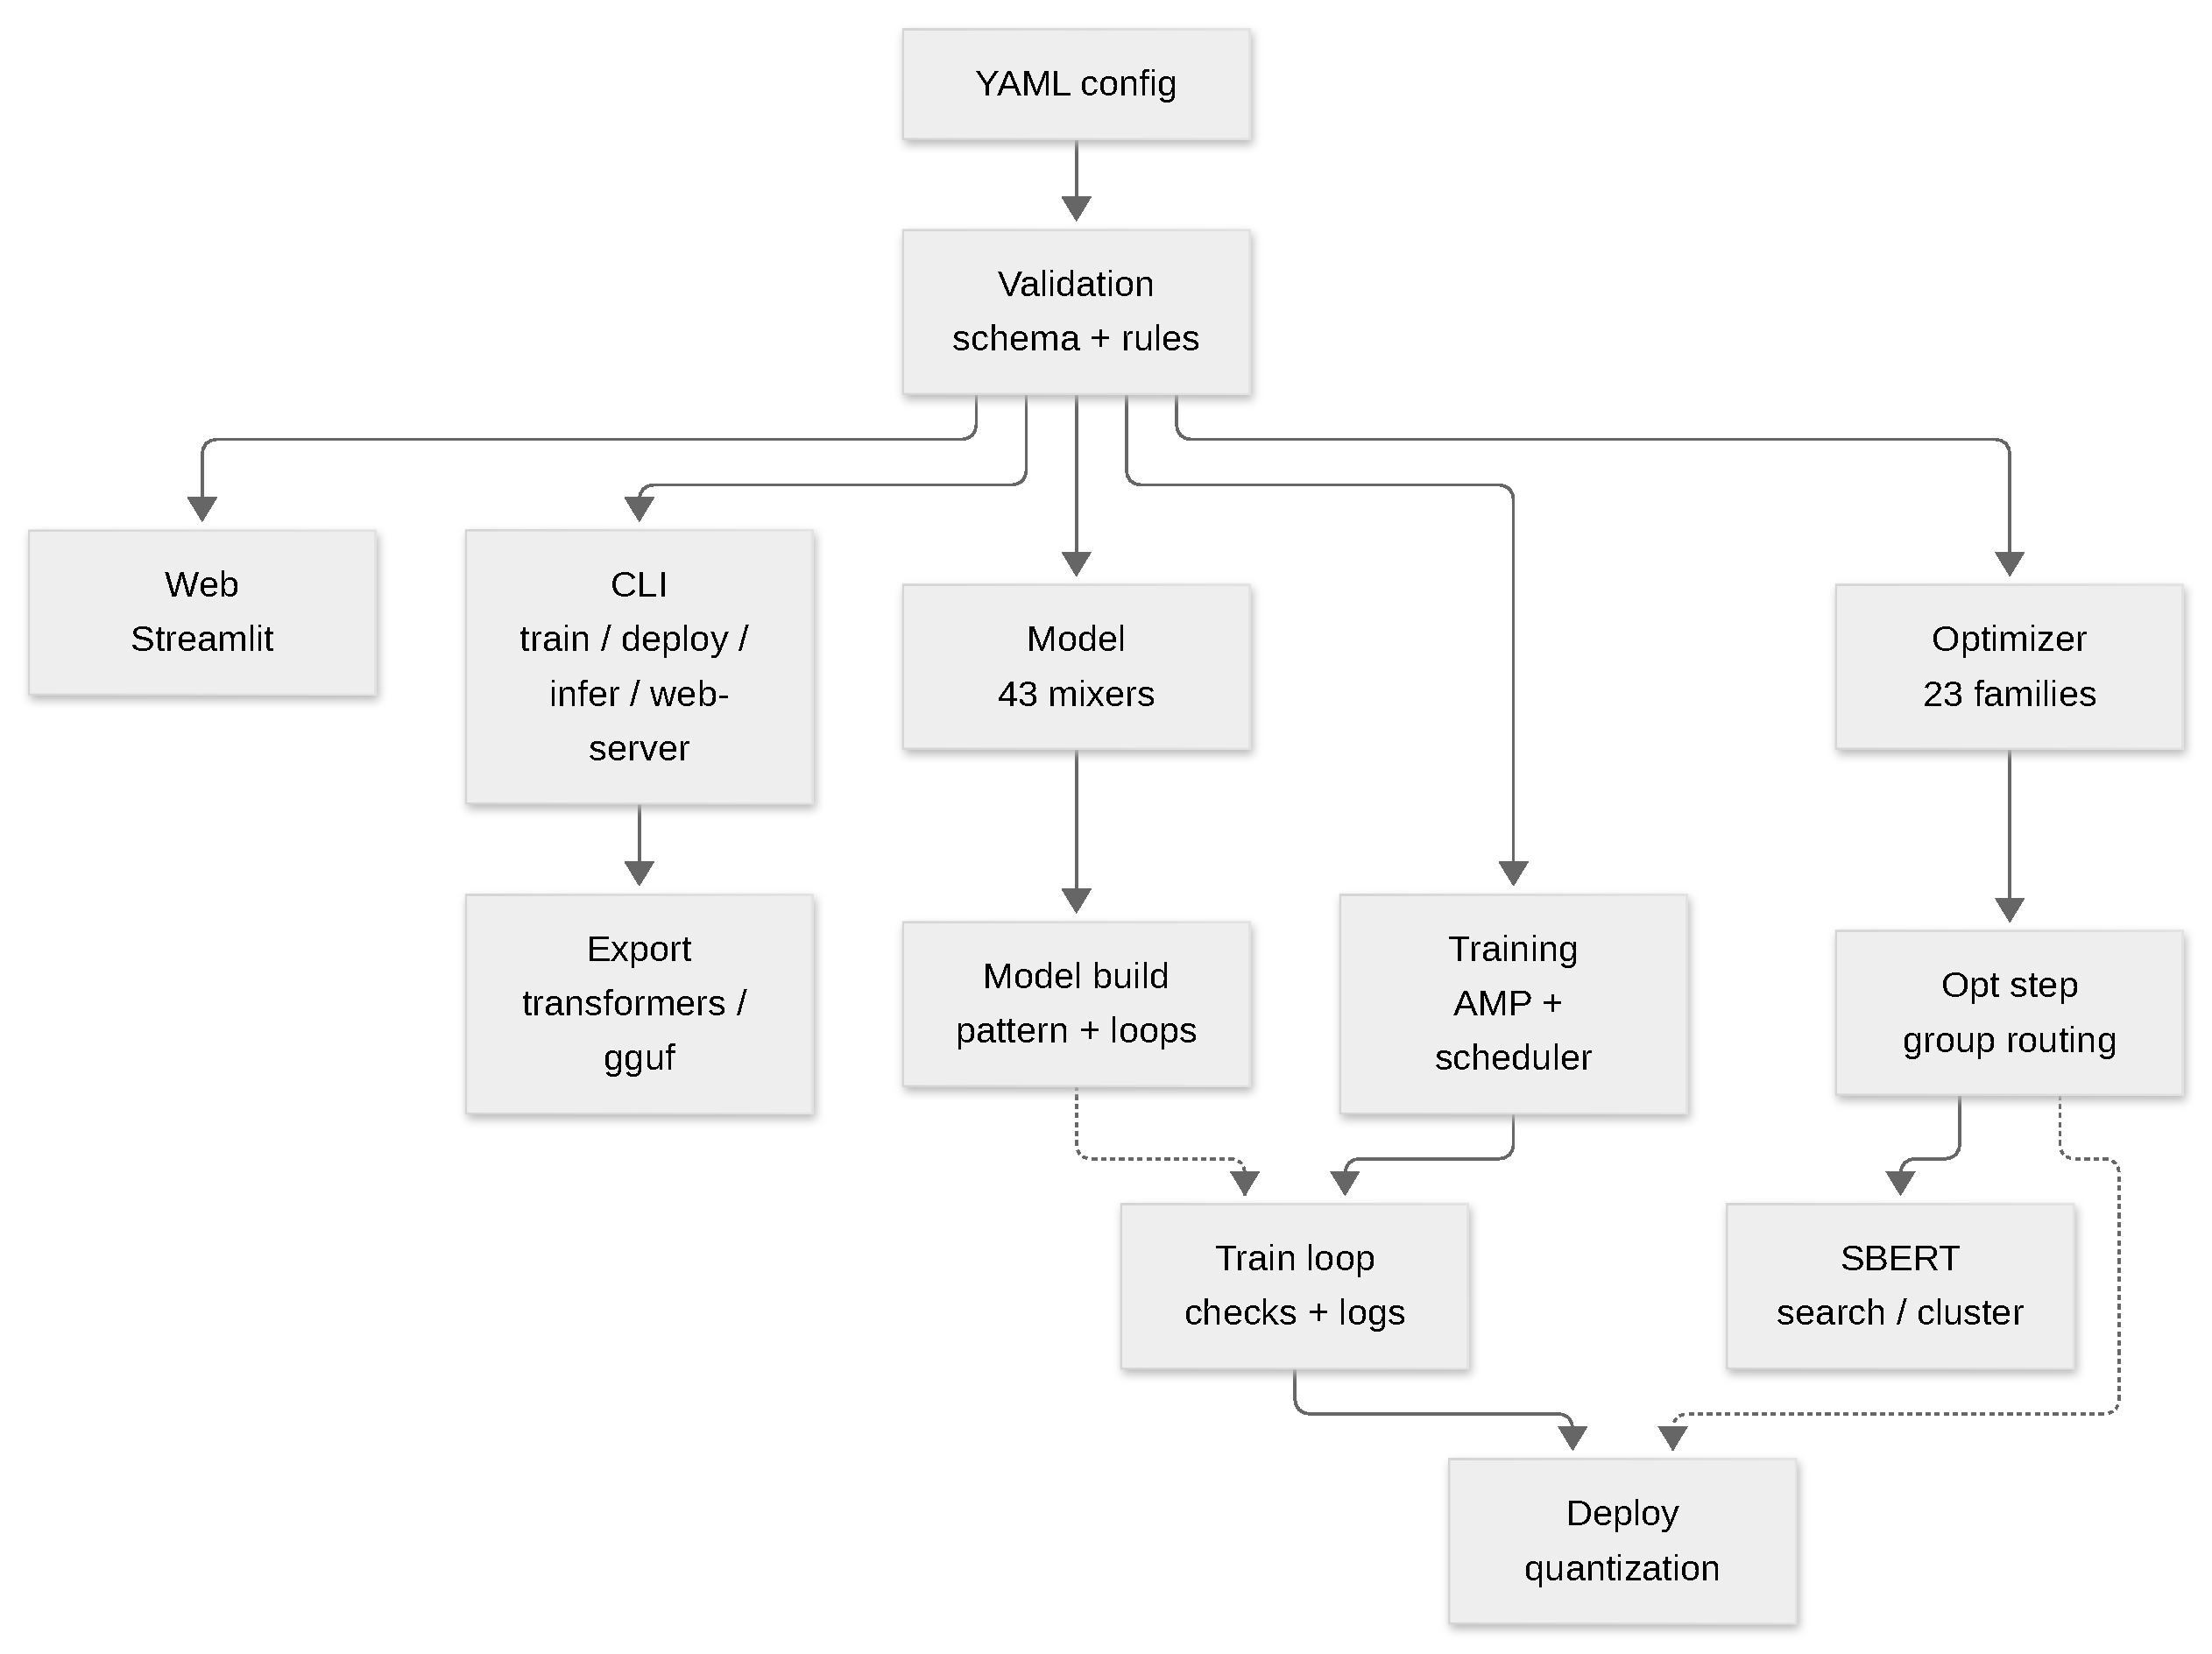
\includegraphics{../paper/figures/system-architecture.pdf}}
\caption{Arquitectura del sistema: la configuración pasa por la validación, se particiona en componentes de modelo, entrenamiento y optimizador, se ejecuta en runtime y produce artefactos de despliegue y SBERT.}
\label{fig:system-architecture}
\end{figure}

\subsection{Alcance del Esquema y Reglas de Validación}
\label{sec:schema-validation}

Los objetos de primer nivel y anidados fijan \texttt{additionalProperties: false}, de modo que las claves desconocidas fallan de inmediato en lugar de ignorarse silenciosamente. Los parámetros del optimizador se restringen además mediante reglas de prefijo por familia. La validación entre componentes rechaza combinaciones incompatibles antes del entrenamiento: el tamaño oculto debe ser divisible por el número de cabezas, el número de cabezas clave--valor debe dividir el número de cabezas, el tamaño del vocabulario debe coincidir con el tokenizer, un modelo base requiere una tarea y (para MLM) un tokenizer, cada tarea requiere su bloque de optimizador correspondiente, las banderas de routers de BitNet requieren BitNet habilitado, y las clases decoder y de visión fuerzan sus respectivos modos de enmascaramiento.

\subsection{Esquema de Configuración}
El esquema completo---campos, tipos, rangos y reglas de validación---se documenta en el Apéndice~\ref{sec:annex-schema}. Los bloques en bucle se configuran con \texttt{num\_layers} y \texttt{num\_loops}, lo que da \texttt{num\_layers}$\times$\texttt{num\_loops} capas lógicas con un conteo de parámetros fijo.

\subsection{Tareas de Entrenamiento}

\texttt{training.task} selecciona el objetivo: \texttt{mlm} (masked language modeling), \texttt{causal\_lm} (predicción autorregresiva de siguiente token, solo clase decoder), \texttt{sbert} (embeddings de oraciones), \texttt{text\_classification} (solo clase encoder) y las tareas de visión \texttt{patch\_prediction}, \texttt{classification} y \texttt{segmentation} (solo Vision Transformer). Las tareas de NLP consumen \texttt{text\_dataset}; las de visión consumen \texttt{vision\_dataset}. Los flujos de embeddings de oraciones se describen en la Sección~\ref{sec:sbert}.

\subsection{Seguridad de Entrenamiento y Semántica de Runtime}

El paso de entrenamiento acumula gradientes sobre micro-lotes, recorta la norma global, verifica desbordamientos posteriores al recorte, reintenta un número acotado de veces ante valores no finitos, despacha el scheduler configurado y rota checkpoints rodantes y del mejor modelo. Cuando \texttt{training.test\_percentage} es positivo, una fracción determinista del dataset se reserva antes del entrenamiento y los pesos finales se evalúan sobre ella; la pérdida y la precisión de la tarea (tasa de error de caracteres para ASR) se escriben en \texttt{test\_metrics.json}. El pseudocódigo completo y la formulación de la partición se remiten al Apéndice~\ref{sec:annex-norm-bitnet-mod}.

\subsection{Variantes de Normalización}
\label{sec:normalization}

La normalización es a la vez una decisión de modelado y una cuestión de compatibilidad del esquema. Los valores aceptados de \texttt{norm.type} son \texttt{layer\_norm}, \texttt{dynamic\_tanh}, \texttt{derf}, \texttt{rms\_norm}, \texttt{prms\_norm} (RMSNorm parcial) y \texttt{flash\_norm} (RMSNorm sin pesos). Sus formulaciones y comparación se detallan en el Apéndice~\ref{sec:annex-norm-bitnet-mod}.

\subsection{Arquitecturas de Flujo Residual}
\label{sec:residual-stream}

Las conexiones residuales se exponen como una decisión de macro-diseño mediante el bloque \texttt{model.residuals}:
\begin{itemize}[leftmargin=*]
    \item \textbf{Estándar}: el residual de identidad clásico \citep{he_deep_2016}.
    \item \textbf{Ninguno}: sin conexión de salto, conservado solo como sonda de ablación.
    \item \textbf{Attention Residuals} (\texttt{full\_attn} o \texttt{block\_attn}): atención aprendida sobre la profundidad que reemplaza la suma residual fija, ya sea sobre todas las capas anteriores o sobre resúmenes por bloques \citep{sun_attnres_2026}.
    \item \textbf{Hiper-conexiones con restricción de variedad} (\texttt{mhc.enabled}): un residual de $n$ flujos cuya matriz de mezcla se restringe al politopo de Birkhoff \citep{xie_mhc_2025}.
\end{itemize}

Attention Residuals se compone con mHC y Mixture-of-Depths; las formulaciones, el cableado y los resultados reportados se recopilan en los Apéndices~\ref{sec:annex-attnres} y~\ref{sec:annex-mhc}.
